\section{文献综述}

\subsection{章的标题}

\bullshit

\subsubsection{节的标题}

\bullshit

\paragraph{小标题}

\bullshit

\newpage
\subsection{国内外研究现状}

\bullshit

\subsubsection{研究方向及进展}

\bullshit

\subsubsection{存在问题}

\bullshit

\newpage
\subsection{研究展望}

\bullshit

这是一个引用示例\cite{vaswani2017attention}。

这是一个图片示例,如图\ref{fig:apple}所示。

\begin{figure}[htbp]
    \centering
    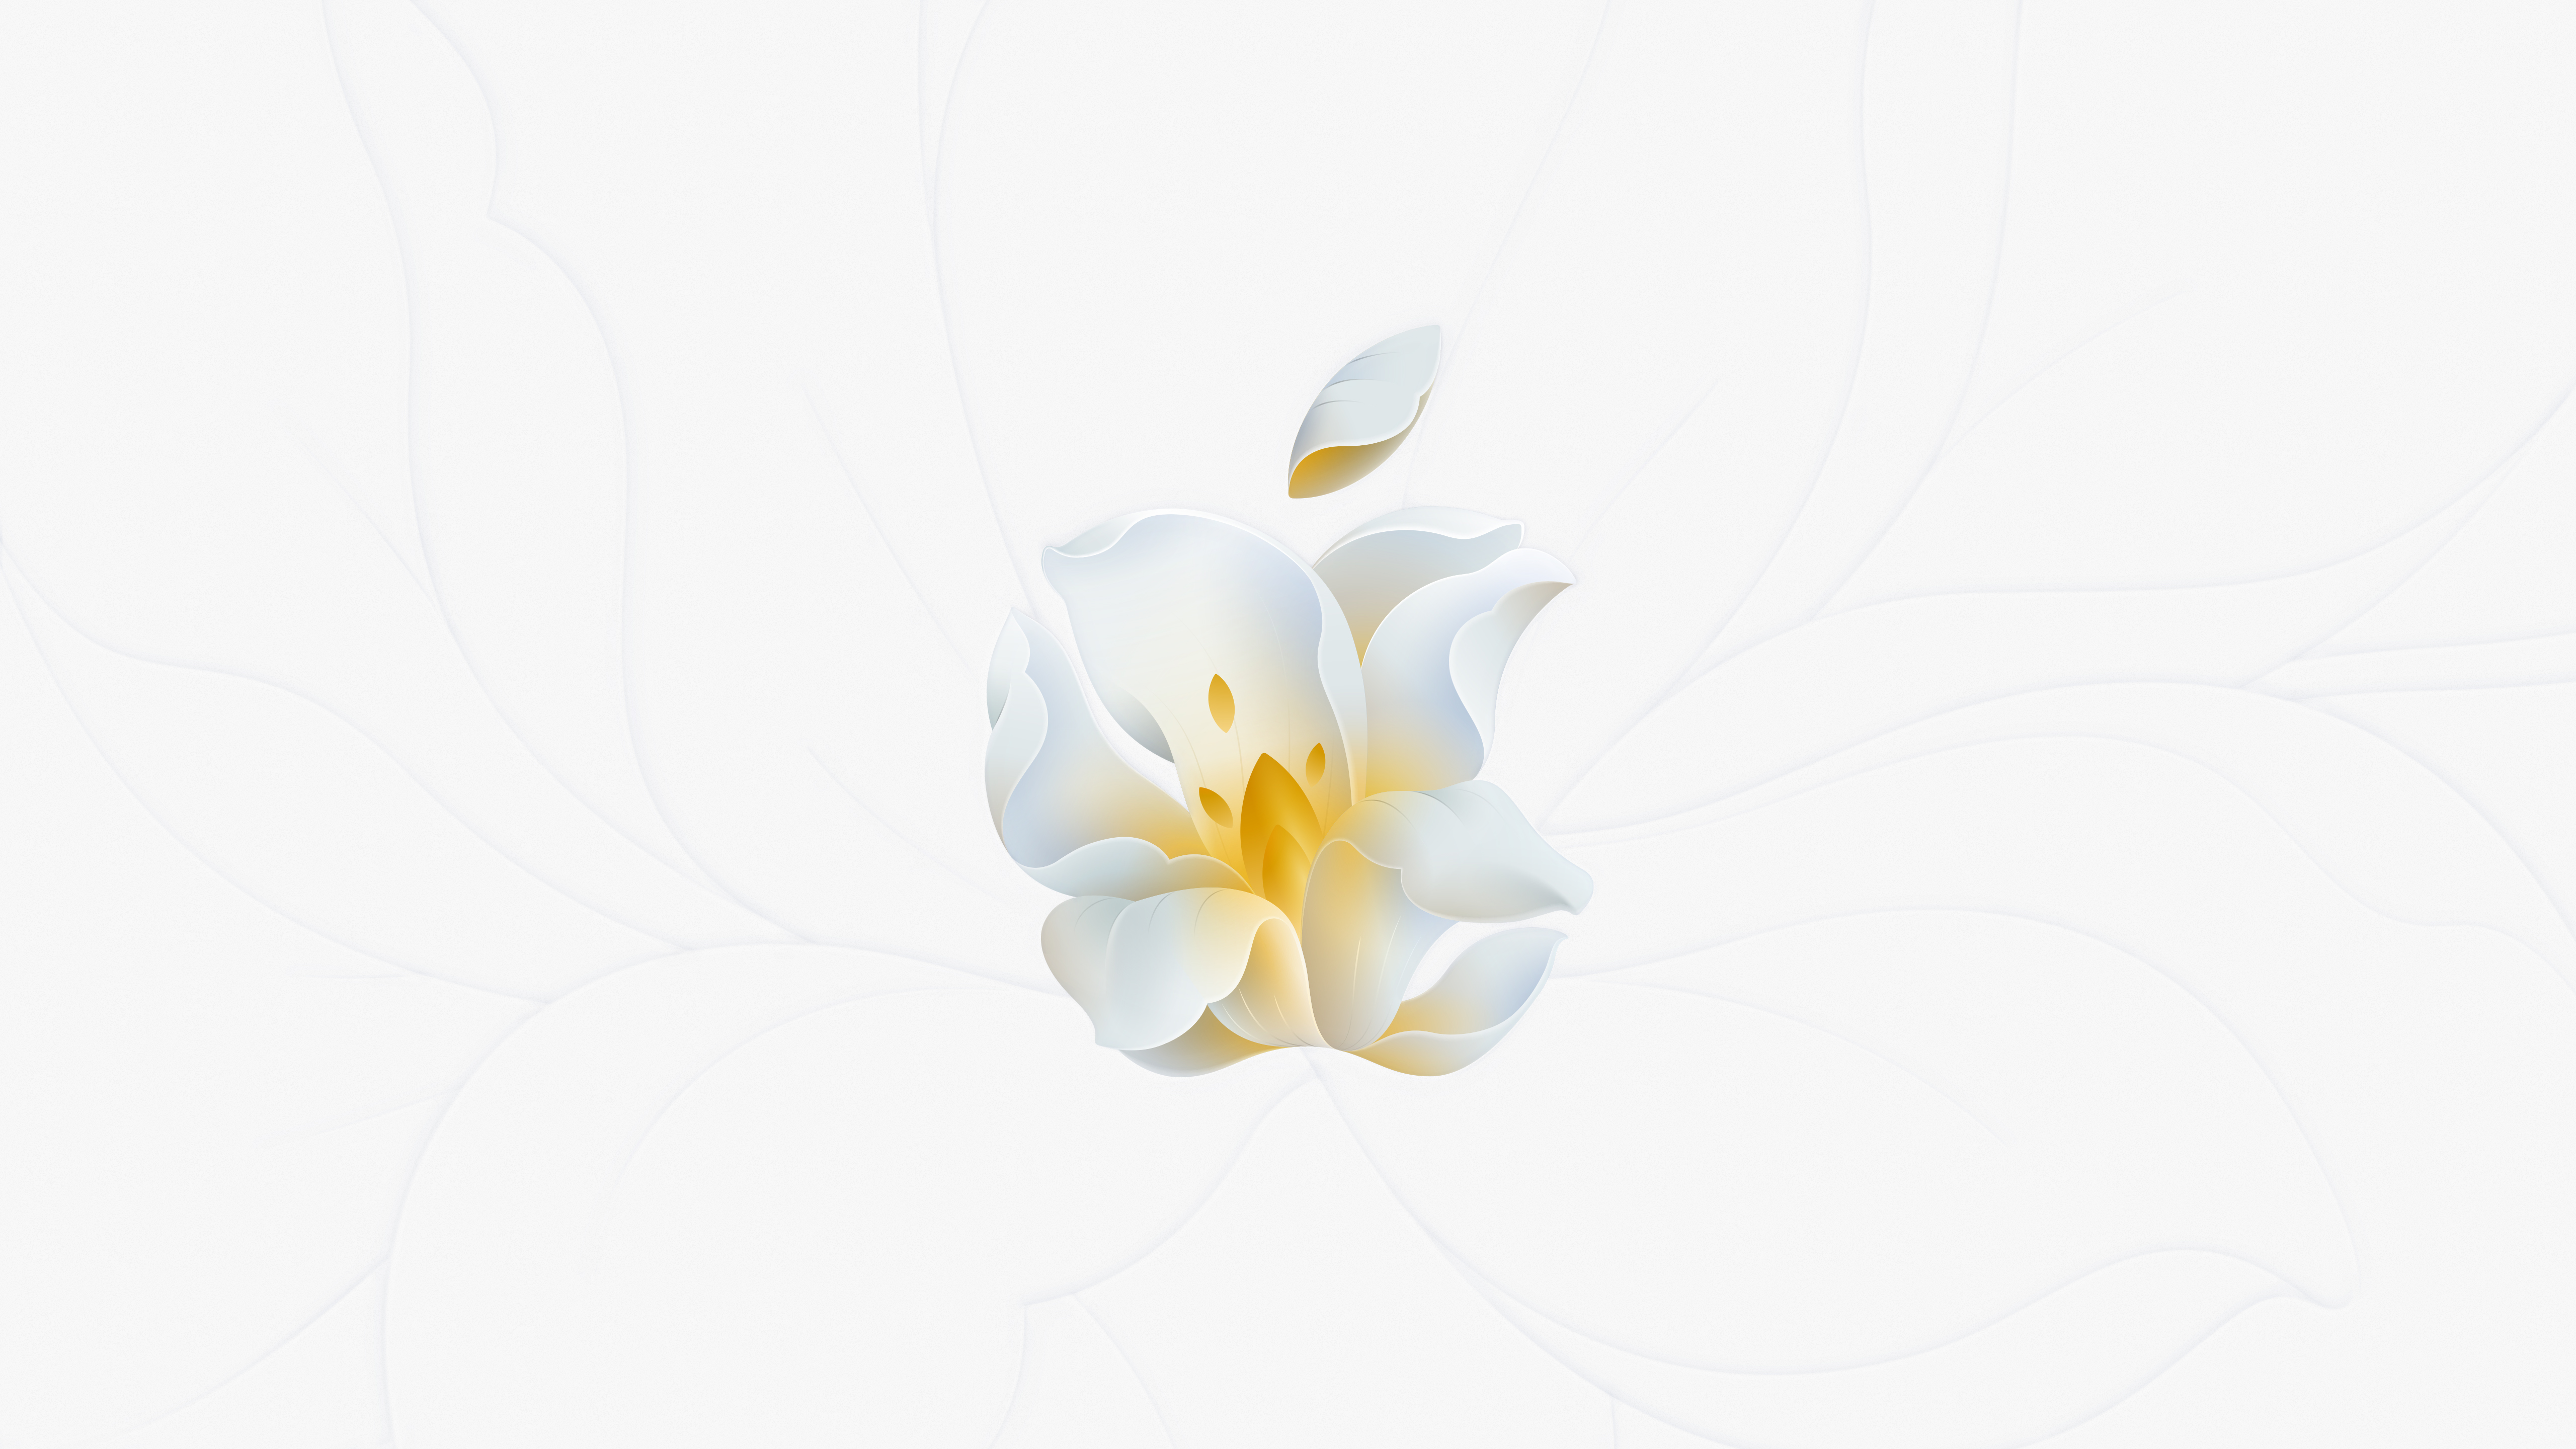
\includegraphics[width=0.8\textwidth]{figs/01/Apple_JingAn_Wallpaper_Mac.jpg}
    \caption{\ptheadingfont{这是一张图}}
    \label{fig:apple}
\end{figure}

这是一个列表示例。

\begin{itemize}
    \item 项目1
    \item 项目2
\end{itemize}

这是一个列表示例,如表\ref{tab:exp}所示。

\begin{table}[htbp]
    \centering
    \caption{\ptheadingfont{这是一个表格}}
    \label{tab:exp}
    \begin{tabular}{|c|c|c|}
        \hline
        x & xx & xxx \\
        \hline
        xxx & xx & x \\
        \hline
    \end{tabular}
\end{table}

% 参考文献
{
\newpage
\bibliographystyle{gbt7714-numerical}
\phantomsection
\subsection{参考文献}
{\normalfont\CJKfamily{simsun}\zihao{5}\setlength{\baselineskip}{14pt}
\renewcommand{\refname}{\vspace{-\baselineskip}}
\bibliography{refs/01_Review}}
}